\section{Definition of Points in Space}

\bx{Find $A + B, A-B, 3A, -2B$ in each of the following cases. 
Draw the points of Exercises 1 and 2 on a sheet of graph paper. 
\en{
\item $A = (2, -1), B = (-1, 1)$
\begin{Solution}

\begin{center}
\begin{tblr}{
  colspec={|Q[50pt, c]|Q[50pt, c]|Q[50pt, c]|Q[50pt, c]|}, 
  row{1-2}={ht=1.4em}, 
  hlines, 
  vlines, 
  width=0.9\textwidth, 
}
$A + B$ & $A - B$ & $3A$ & $-2B$ \\
$(1,0)$ & $(3,-2)$ & $(6,-3)$ & $(2,-2)$ \\
\end{tblr}
\end{center}

\begin{center}
  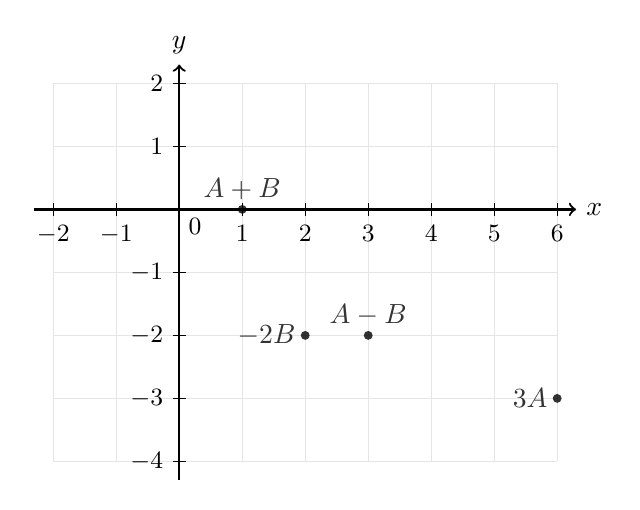
\begin{tikzpicture}[scale=0.8]
  \draw[gray!20, step=1cm] (-2,-4) grid (6,2); 
  \draw[->, thick] (-2.3,0) -- (6.3,0) node[right] {$x$};
  \draw[->, thick] (0,-4.3) -- (0,2.3) node[above] {$y$};

  \foreach \x in {-2,-1,...,6} {
    \ifnum\x=0
      \draw (\x,0.1) -- (\x,-0.1); 
    \else
      \draw (\x,0.1) -- (\x,-0.1) node[below] {\small$\x$}; 
    \fi
  }

  \foreach \y in {-4,-3,...,2} {
    \ifnum\y=0
      \draw (0.1,\y) -- (-0.1,\y); 
    \else
      \draw (0.1,\y) -- (-0.1,\y) node[left] {\small$\y$}; 
    \fi
  }

  \node[anchor=base, xshift=0.2cm, yshift=-0.08cm, font=\small] at (0,-0.3cm) {$0$};

  \fill[black, opacity=0.8] (1,0) circle (2pt) node[above] {$A+B$};
  \fill[black, opacity=0.8] (3,-2) circle (2pt) node[above] {$A-B$};
  \fill[black, opacity=0.8] (6,-3) circle (2pt) node[left] {$3A$};
  \fill[black, opacity=0.8] (2,-2) circle (2pt) node[left] {$-2B$};
\end{tikzpicture}
\end{center}
\end{Solution}

\newpage

\item $A(-1, 3), B(0, 4)$
\begin{Solution}

\begin{center}
\begin{tblr}{
  colspec={|Q[50pt, c]|Q[50pt, c]|Q[50pt, c]|Q[50pt, c]|}, 
  row{1-2}={ht=1.4em}, 
  hlines, 
  vlines, 
  width=0.9\textwidth, 
}
$A + B$ & $A - B$ & $3A$ & $-2B$ \\
$(-1, 7)$ & $(-1, -1)$ & $(-3, 9)$ & $(0, -8)$ \\
\end{tblr}
\end{center}

\begin{center}
  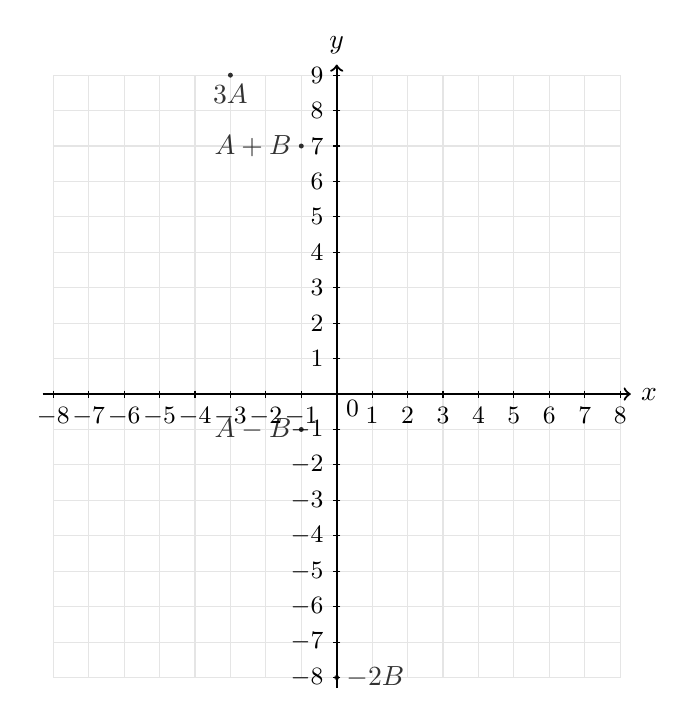
\begin{tikzpicture}[scale=0.45]
  \draw[gray!20, step=1cm] (-8,-8) grid (8,9); 
  \draw[->, thick] (-8.3,0) -- (8.3,0) node[right] {$x$};
  \draw[->, thick] (0,-8.3) -- (0,9.3) node[above] {$y$};

  \foreach \x in {-8,-7,...,8} {
    \ifnum\x=0
      \draw (\x,0.1) -- (\x,-0.1); 
    \else
      \draw (\x,0.1) -- (\x,-0.1) node[below] {\small$\x$};
    \fi
  }

  \foreach \y in {-8,-7,...,9} {
    \ifnum\y=0
      \draw (0.1,\y) -- (-0.1,\y); 
    \else
      \draw (0.1,\y) -- (-0.1,\y) node[left] {\small$\y$}; 
    \fi
  }

  \node[anchor=base, xshift=0.2cm, yshift=-0.15cm, font=\small] at (0,-0.3cm) {$0$};

  \fill[black, opacity=0.8] (-1,7) circle (2pt) node[left] {$A+B$};
  \fill[black, opacity=0.8] (-1,-1) circle (2pt) node[left] {$A-B$};
  \fill[black, opacity=0.8] (-3,9) circle (2pt) node[below] {$3A$};
  \fill[black, opacity=0.8] (0,-8) circle (2pt) node[right] {$-2B$};
\end{tikzpicture}
\end{center}
\end{Solution}

\item $A(2, -1, 5), B(-1, 1, 1)$
\begin{Solution}
\begin{center}
\begin{tblr}{
  colspec={|Q[50pt, c]|Q[50pt, c]|Q[50pt, c]|Q[50pt, c]|}, 
  row{1-2}={ht=1.4em}, 
  hlines, 
  vlines, 
  width=0.9\textwidth, 
}
$A + B$ & $A - B$ & $3A$ & $-2B$ \\
$(1, 0, 6)$ & $(3, -2, 4)$ & $(6, -3, 15)$ & $(2, -2, -2)$ \\
\end{tblr}
\end{center}
\end{Solution}

\item $A(-1, -2, 3), B(-1, 3, -4)$
\begin{Solution}
\begin{center}
\begin{tblr}{
  colspec={|Q[50pt, c]|Q[50pt, c]|Q[50pt, c]|Q[50pt, c]|}, 
  row{1-2}={ht=1.4em}, 
  hlines, 
  vlines, 
  width=0.9\textwidth, 
}
$A + B$ & $A - B$ & $3A$ & $-2B$ \\
$(-2, 1, -1)$ & $(0, -5, 7)$ & $(-3, -6, 9)$ & $(2, -6, 8)$ \\
\end{tblr}
\end{center}
\end{Solution}

\newpage

\item $A(\pi, 3, -1), B(2 \pi, -3, 7)$
\begin{Solution}
\begin{center}
\begin{tblr}{
  colspec={|Q[50pt, c]|Q[50pt, c]|Q[50pt, c]|Q[50pt, c]|}, 
  row{1-2}={ht=1.4em},
  hlines,
  vlines,
  width=0.9\textwidth, 
}
$A + B$ & $A - B$ & $3A$ & $-2B$ \\
$(3\pi, 0, 6)$ & $(-\pi, 6, -8)$ & $(3\pi, 9, -3)$ & $(-4\pi, 6, -14)$ \\
\end{tblr}
\end{center}
\end{Solution}

\item $A(15, -2, 4), B(\pi, 3, -1)$
\begin{Solution}
\begin{center}
\begin{tblr}{
  colspec={|Q[50pt, c]|Q[50pt, c]|Q[50pt, c]|Q[50pt, c]|}, 
  row{1-2}={ht=1.4em},
  hlines,
  vlines,
  width=0.9\textwidth, 
}
$A + B$ & $A - B$ & $3A$ & $-2B$ \\
$(15 + \pi, 1, 3)$ & $(15-\pi, -5, 5)$ & $(45, -6, 12)$ & $(-2\pi, -6, 2)$ \\
\end{tblr}
\end{center}
\end{Solution}


}
}